%!TEX root = Main.tex
\documentclass[Main]{subfiles}

\begin{document}

\section{Robot Mechanics} % (fold)
	\label{sec:robot_mechanics}

	\subsection{Chassis} % (fold)
	\label{sub:chassis}
		The chassis of the robot is a Baron-4WD mobile platform bought from the website dfrobots.com. 
		It consist of a lower frame where up to four DC motors can be attached, and a top plate with holes for mounting of other devices. 
		\autoref{fig:baron_platform} shows a picture of the chassis where it is assembled with the default package items from dfrobots.
		\begin{figure}[H]
			\centering
			\begin{subfigure}[b]{0.55\linewidth}
				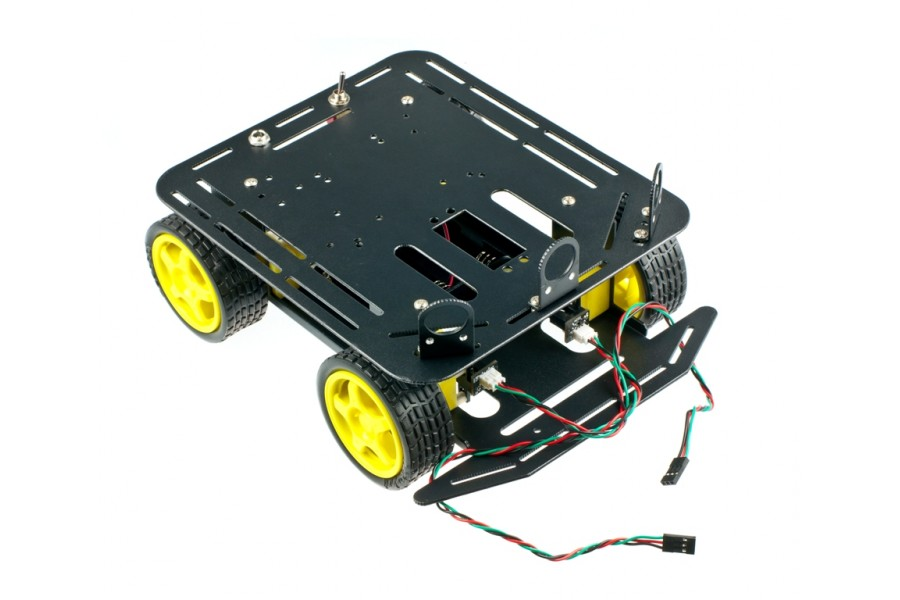
\includegraphics[width=1\linewidth]{./Figures/baron_platform.jpg}
				\caption{The Baron-4WD platform}
				\label{fig:baron_platform}
			\end{subfigure}	
			\begin{subfigure}[b]{0.4\linewidth}
				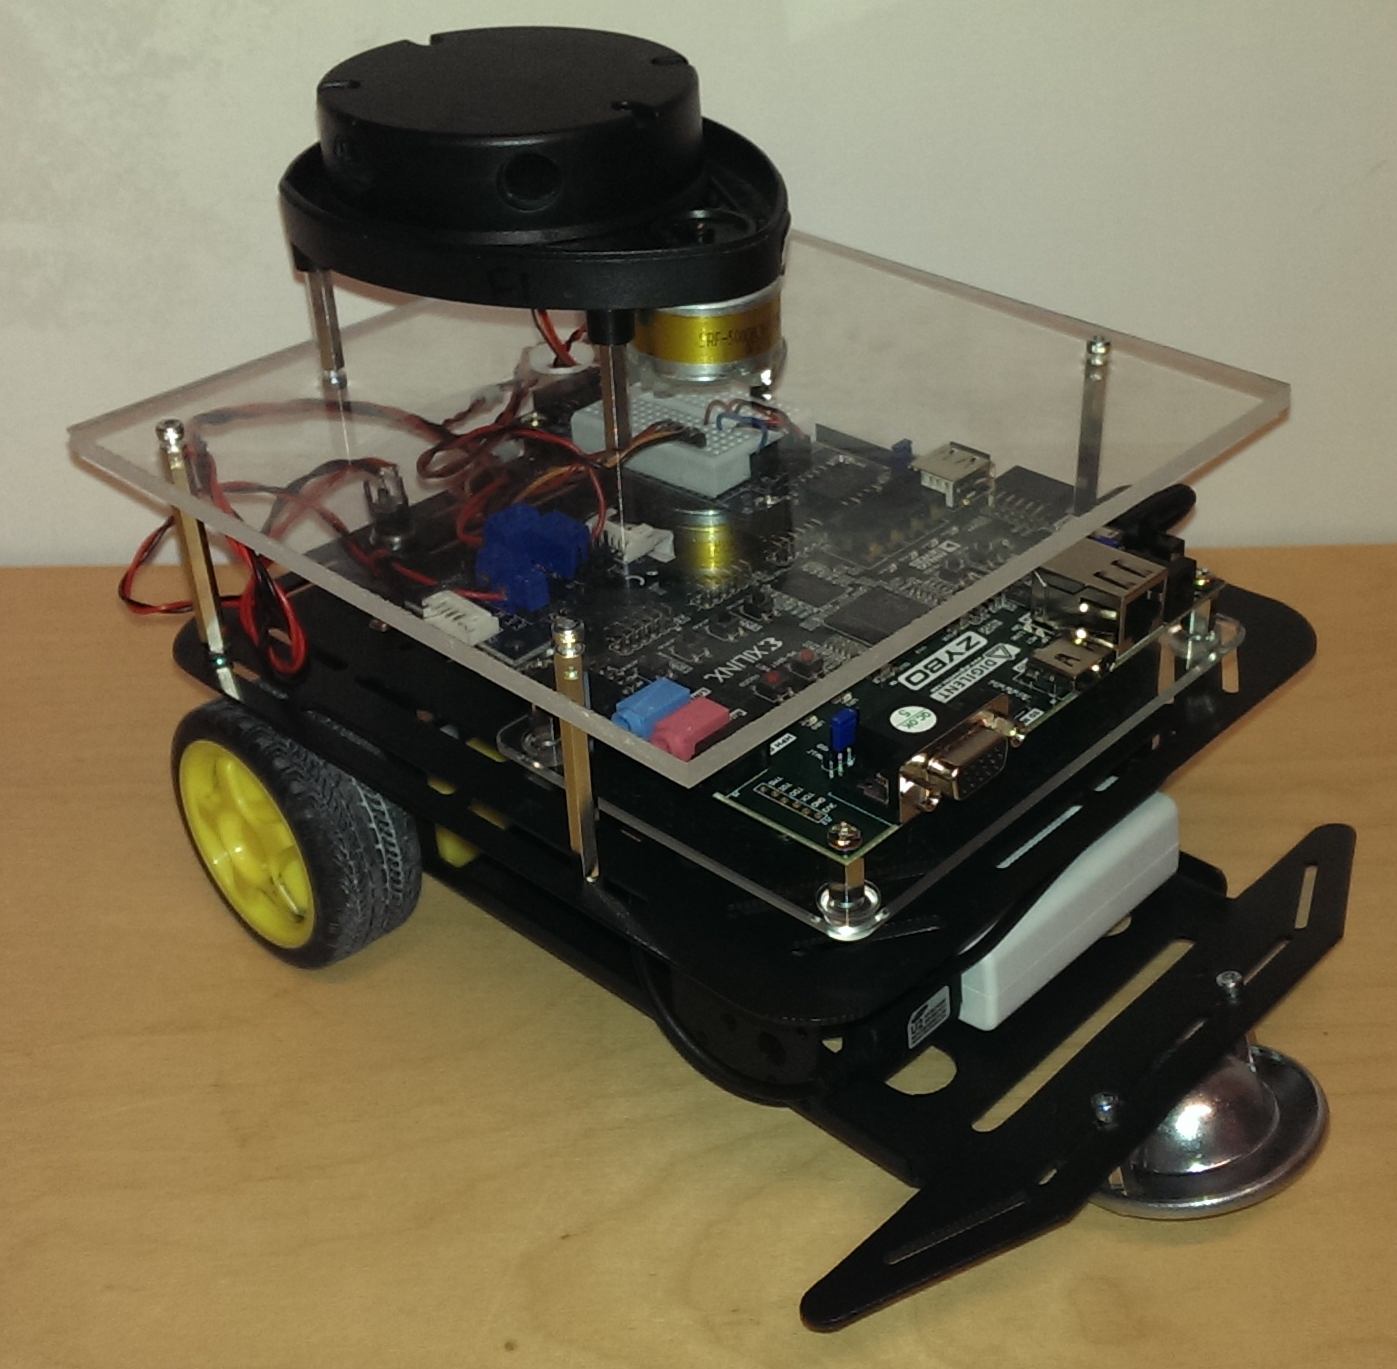
\includegraphics[width=1\linewidth]{./Figures/final_robot.png}
				\caption{The final robot configuration}
				\label{fig:final_robot}
			\end{subfigure}
		\caption{}
		\label{fig:robots}
		\end{figure}
		In this project it was decide to only use two motors at the rear end of the chassis to make a simpler motion model for the robot; more about the motion model in \autoref{sub:motion_model}. 
		Instead of front wheels, a ball caster was attach to insure the turning ability. 
		By only using motors in the rear end, the lower frame had a lot of room where the power supplies could be place and thereby leaving the top plate free for the processing platform, a Zynq development board, \autoref{sub:platform}, and mounting of the sensors. 
		The sensor used in this project is, as mentioned earlier, a LIDAR which required a specific mounting pattern, that filled out most of the top plate's area, thereby only leaving a small area for the ZYBO. 
		More about the LIDAR in \autoref{sub:sensor}.
		The LIDAR was therefore mounted on a acrylic plate which then was mounted on top of the top plate. 
		The final robot configuration is shown in \autoref{fig:final_robot}.
		
		% subsection chassis (end)

	\subsection{Motor characteristics} % (fold)
	\label{sub:motor_characteristics}

		

		\begin{figure}[H]
			\centering
			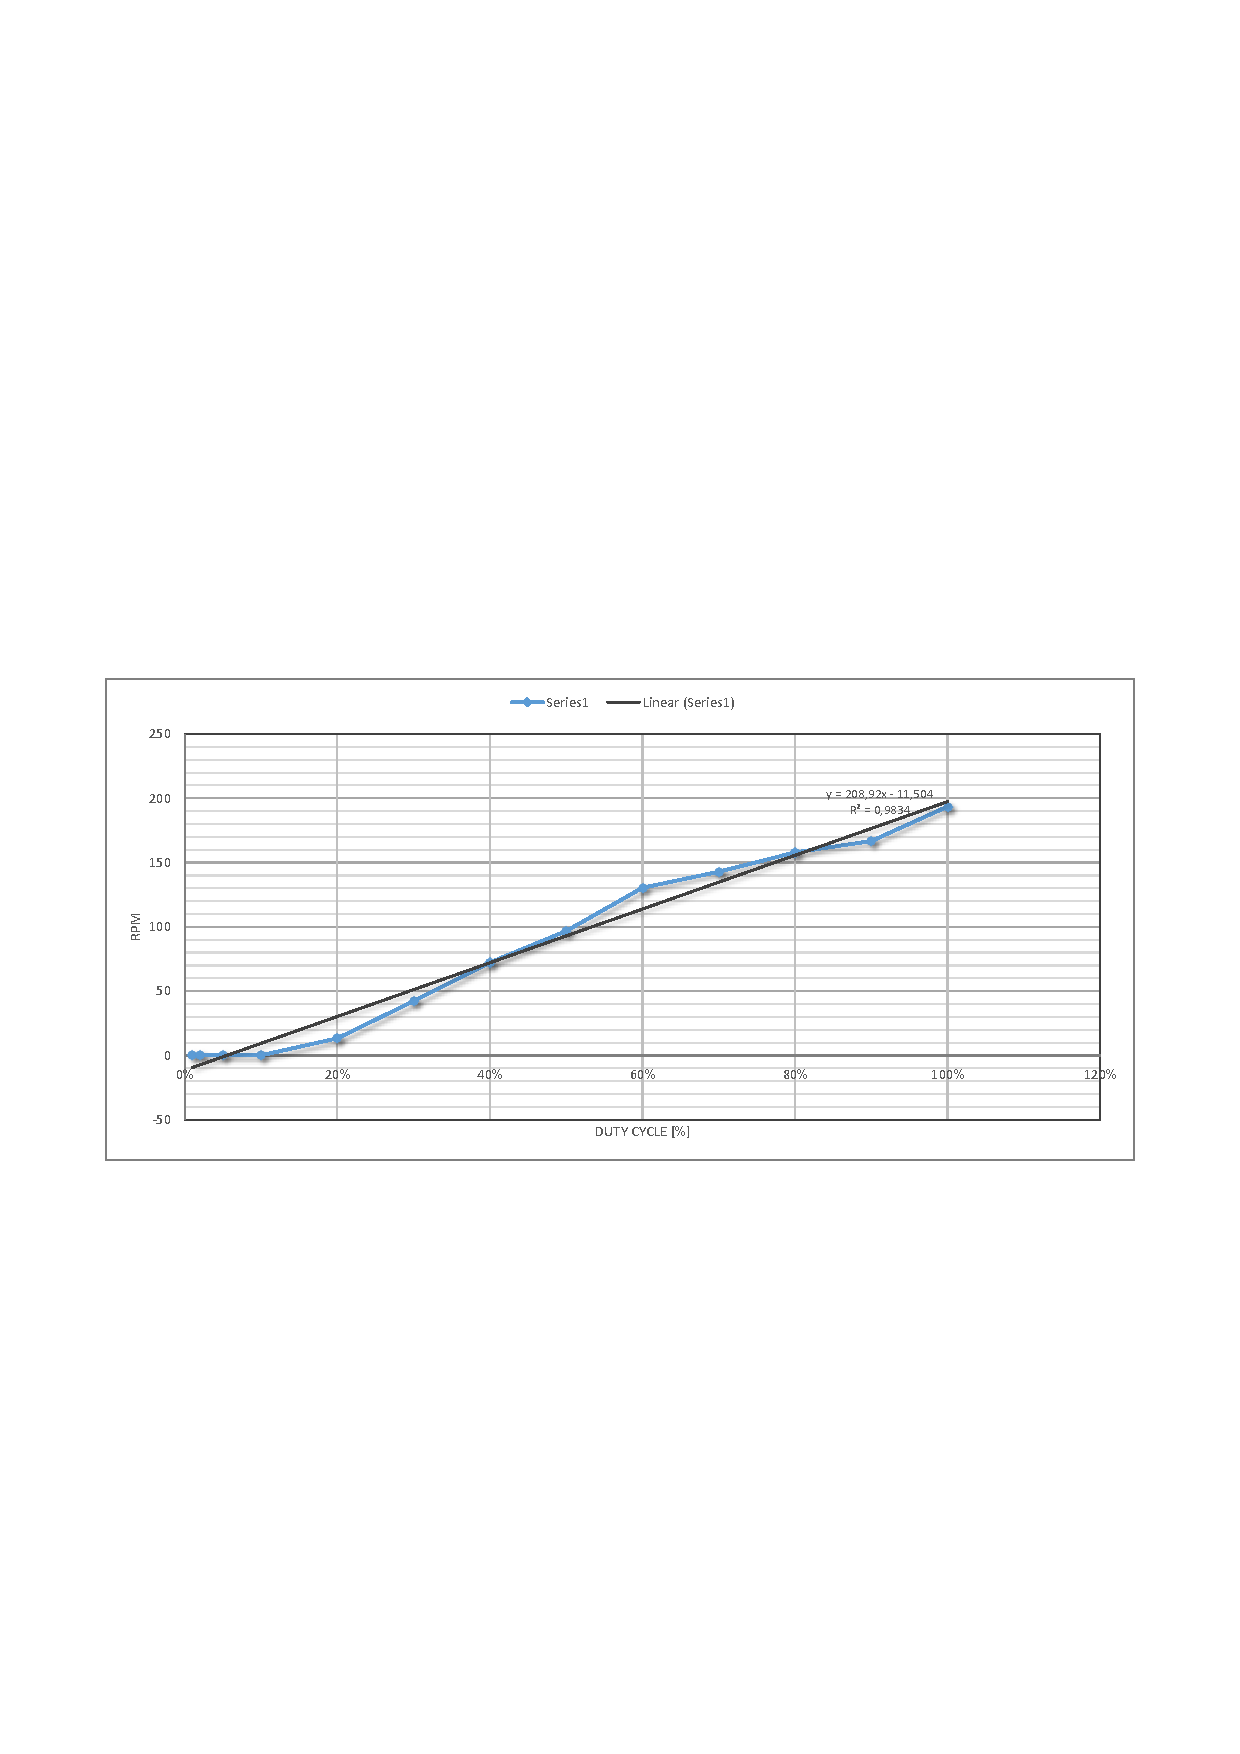
\includegraphics[width=\linewidth]{MotorSpeedTest}
			\caption{Motor rotational velocity [RPM] vs. PWM duty cycle [\%]}
			\label{fig:motor_speed_test}
		\end{figure}
		
		% motor characteristics (end)

	\subsection{Motion model} % (fold)
	\label{sub:motion_model}

		The motion model used in this project is based on a simple rotation and the move model.
		The rotation is however not just a change in orientation since the robot is not rotating around it's center of mass, but around one of it's wheels.
		This means that during rotation the center of mass is also being moved.
		The difference between these two rotations is shown in \autoref{fig:motion_models}.
		\begin{figure}[H]
			\centering
			\begin{subfigure}[b]{0.45\linewidth}
				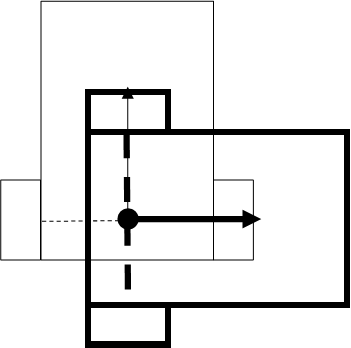
\includegraphics[scale=0.8]{./Figures/motion_model1.png}
				\caption{Around center of mass}
				\label{fig:motion_model1}
			\end{subfigure}	
			\begin{subfigure}[b]{0.45\linewidth}
				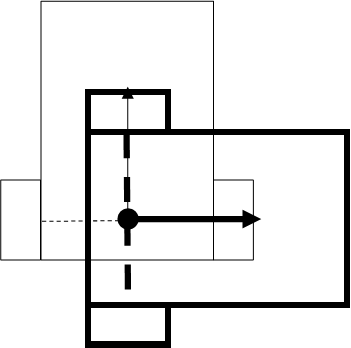
\includegraphics[scale=0.8]{./Figures/motion_model2.png}
				\caption{Around wheel}
				\label{fig:motion_model2}
			\end{subfigure}
		\caption{Rotation models}
		\label{fig:motion_models}
		\end{figure}
		Where the thin lined figures are the robot before rotation, and the thick figures are after.

		To describe how the center of mass is being move when turning around the wheel, the following equation from \cite{Wikipedia2015} is used, which is just a 2D rotation matrix.
		\begin{equation}
		\begin{bmatrix} x' \\ y' \end{bmatrix} = \begin{bmatrix} \cos{\theta} & -\sin{\theta} \\ \sin{\theta} & \cos{\theta} \end{bmatrix} \begin{bmatrix} x \\ y \end{bmatrix}
		\end{equation}
		In this equation $x$ and $y$ are the coordinates before the transformation, $x'$ and $y'$ are after transformation, and $\theta$ is the angle of how much the orientation is being changed.

		The movement is described simple by the change in the coordinates, \autoref{eq:translation_matrix}.
		\begin{equation}
		\label{eq:translation_matrix}
		\begin{bmatrix} x' \\ y' \end{bmatrix} = \begin{bmatrix}  d & 0 & x \\ 0 & d & y \end{bmatrix} \begin{bmatrix} \cos{\phi} \\ \sin{\phi} \\ 1 \end{bmatrix} 		
		\end{equation}
		Where $x$, $y$, $x'$ and $y'$ is the same as previous, $\phi$ is the orientation and $d$ is the distance of the movement.
		In this equation it is obvious to see that it is assumed that the robot moves with constant velocity.
		This means that it is assumed that the motors can produce the correct velocity in a step response.

		It was chosen to use this discrete model, where rotation and translation (movement) are done separately, above a continues model, where rotation is being done while translating \fxnote{er det rigtigt}.
		The reason for this was to keep model motion as simple as possible to begin with, and then extend it when a functional robot was made.
		To extend the model to continues would require that the motors are controlled by PI or PID controllers instead of just a simple PWM signal.

		Again for simplicity, it was decide that the change in orientation were constrainted to be in intervals of $90\degree$.
		This meant that the robot in theory only should be able to drive horizontal and vertical in the grid map. \fxnote{måske lidt bedre formulering tak:S}

		% subsection motion_model (end)

	% subsection robot_mechanics (end)

\end{document}